\documentclass[]{article}
\author{Diego Biagini}
\title{Componenti connesse di un grafo e \\alberi di connessione minimi}
\date{}

\usepackage[utf8]{inputenc}
\usepackage[margin=3cm]{geometry}
\usepackage{algorithmic}
\usepackage{algorithm}
\usepackage{graphicx}
\usepackage{amsmath}
\floatname{algorithm}{}
\usepackage{caption, subcaption}
    \captionsetup[sub]{labelformat=simple}
    \renewcommand{\thesubfigure}{(\alph{subfigure})} % Style: 1(a), 1(b)
\graphicspath{{../plots/}}


\begin{document}
\maketitle
\section{Introduzione}
Il grafo è una struttura che ha numerose applicazioni sia nei campi dell'informatica sia in quelli dell'ottimizzazione.\\
Alcuni tipi di operazioni possibili su di essi sono le visite e la ricerca di cammini, o insiemi di cammini, particolari.\\
Gli esperimenti che saranno eseguiti serviranno a esaminare due tipi particolari di ricerche in un grafo: la ricerca delle componenti connesse e la ricerca dell'MST(minimum spanning tree), quest'ultima sarà effettuata attraverso l'uso dell'algoritmo di Kruskal.\\
Ciò che ci interesserà scoprire maggiormente è il comportamento degli algoritmi per queste ricerche all'aumentare dei nodi del grafo.\\
\'E necessario infatti che essi siano efficienti su grafi relativamente estesi date le applicazioni reali, un esempio per le componenti connesse è nell'analisi di immagini e quindi OCR, mentre la ricerca di un albero di connessione minimo è un classico problema che si presenta nelle telecomunicazioni.\\ 
\section{Cenni teorici}
\subsection{Grafi}
Un grafo può essere visto come un insieme di elementi in relazione tra loro.\\
Questa relazione è indicata dagli archi che li connettono.\\
Un grafo può essere individuato attraverso due insiemi:
\begin{itemize}
\item l'insieme dei vertici $V$
\item l'insieme degli archi $E$ ,ogni arco è indicato da una coppia di vertici
\end{itemize}
Un grafo si dice \textbf{non diretto} se $E$ è composto da coppie di vertici ordinate.\\
Viene definito \textbf{cammino} di un grafo dal vertice $u$ a $u'$ una sequenza di vertici $<v_0, ... , v_k>$ tale che $v_0 = u,v_k=u'$ e $(v_i-1, v_i)$ è un arco presente in $E$ per $i = 2,..., k-1$.\\
Se $v_0 = v_k$ e il cammino è formato da almeno un arco invece siamo in presenza di un \textbf{ciclo}
\\\\
\'E possibile memorizzare i grafi in diversi modi, due opzioni possibili sono le seguenti:
\begin{itemize}
\item \textbf{Lista di adiacenza}, viene creata una lista per ogni nodo e queste liste contengono gli altri nodi a cui è collegato
\item \textbf{Matrice di adiacenza}, si memorizza una matrice $A \in (|V| \times |V|)$, se esiste un arco tra il nodo i-esimo e j-esimo allora $a_{ij} = 1$, altrimenti $a_{ij} = 0$. 
\end{itemize}
Ognuna di queste rappresentazioni ha certi vantaggi minori rispetto alle altre, per esempio con una lista viene usata in genere meno memoria ma cercare se un certo nodo è collegato ad un altro diventa più difficoltoso.\\ 
E' possibile visitare un grafo in numerosi modi, le due visite che hanno più usi sono la \textbf{BFS}(Breadth first search) e la \textbf{DFS}(Depth first search).\\
\subsection{Strutture dati per insiemi disgiunti}
Si occupano di gestire un qualsiasi numero di insiemi dinamici contenenti elementi di vario tipo.\\
Per identificare ciascun insieme viene scelto un rappresentante.\\
Le operazioni che devono essere garantite sono:
\begin{itemize}
\item \textbf{Make-Set(x)}, crea un insieme contenente un solo elemento,x
\item \textbf{Union(x,y)}, fonde due insiemi in modo che il rappresentante di ogni elemento sia lo stesso 
\item \textbf{Find-Set(x)}, restituisce il rappresentante di x
\end{itemize}
Le implementazioni possibili per questa struttura dati sono:
\begin{itemize}
\item attraverso liste, ogni insieme è rappresentato da una lista concatenata e ogni elemento dell'insieme ha un puntatore al rappresentante; qui è possibile usare l'euristica dell'unione pesata
\item attraverso una foresta di alberi, ogni insieme è identificato da un albero, siamo in grado di trovare il rappresentante risalendo l'albero, inoltre viene memorizzato il rango di ogni albero, ovvero la sua altezza; qui è possibile usare l'euristica dell'unione per rango, simile all'unione pesata, e la compressione dei cammini in modo che la scalata dell'albero sia più corta possibile.
\end{itemize}
Usando la rappresentazione con una foresta di alberi e implementando entrambe le sue euristiche siamo in grado di realizzare una struttura dati molto efficiente, infatti l'unione(che è l'operazione più costosa) tra due insiemi di dimensione $m$ e $n$ assume un costo del tipo $O(m\alpha (m,n))$ dove $\alpha$ è la funzione inversa di Ackermann, una funzione che cresce così lentamente da poter essere considerata costante nelle applicazioni reali.\\
Quindi abbiamo che il costo dell'unione è lineare rispetto a $m$.\\
\subsection{Componenti connesse di un grafo}
Dato un grafo $G =(V,E)$ è possibile partizionarlo in dei suoi sottoinsiemi, detti componenti connesse.\\
Una componente connessa può essere vista come relazione di equivalenza tra nodi di un grafo, secondo la relazione "è raggiungibile da".\\
Quindi due nodi $u$ e $v$ appartengono alla stessa componente connessa se e solo se esiste un cammino tra loro.\\
Per trovare le componenti connesse in modo semplice si usa il seguente algoritmo, che fa uso di insiemi disgiunti:
\begin{algorithm}
\caption{Connected-Components(G)}
\begin{algorithmic}[1]
\FOR{ogni vertice $v \in G.V$} 
	\STATE $MAKE\mbox{-}SET(v)$
\ENDFOR 
\FOR{ogni arco $(u,v) \in G.E$}
	\IF{$FIND \mbox{-} SET(u) \neq FIND \mbox{-} SET(v)$}
	\STATE $UNION(u,v)$	
	\ENDIF
\ENDFOR
\end{algorithmic}
\end{algorithm}
\subsection{MST}
Dato un grafo diretto pesato(ogni arco ha un peso $w(u,v)$) e connesso è possibile trovare un albero minimo di connessione.\\
Questo è un sottoinsieme aciclico $T\subseteq E$ che connette tutti i vertici e che ha peso totale minore, ovvero\\
$$w(T) = \sum_{(u,v)\in T} w(u,v)$$ \\
deve essere minimo
\newpage
Tutti gli algoritmi per trovare l'MST di un grafo sono costruiti nel modo seguente:
\begin{algorithm}
\caption{Generic-MST(G)}
\begin{algorithmic}[1]
\STATE $A \leftarrow \emptyset$
\WHILE{A non forma un albero di connessione}
	\STATE {trova un arco $(u,v)$ sicuro per A}
	\STATE {$A \leftarrow A \cup \{(u,v)\}$}
\ENDWHILE
\end{algorithmic}
\end{algorithm}
\\
Per trovare un arco sicuro è utile il seguente teorema:\\
Sia $G=(V,E)$ un grafo non orientato e connesso con un peso associato ad ogni arco. Sia A un sottoinsieme di E contenuto in un qualche MST per G. Sia $(S, V-S)$ un qualunque taglio che rispetta A. Allora se l'arco $(u,v)$ è un arco leggero che attraversa $(S, V-S)$ è un arco sicuro per A.\\\\
Da questo è possibile arrivare a sviluppare l'algoritmo di Kruskal per la ricerca dell'albero di connessione minimo di un grafo:
\begin{algorithm}
\caption{MST-Kruskal(G)}
\begin{algorithmic}[1]
\STATE $A \leftarrow \emptyset$
\FOR{ogni vertice $v \in G.V$} 
	\STATE $MAKE\mbox{-}SET(v)$
\ENDFOR 
\STATE Ordina gli archi in senso non decrescente rispetto al peso $w$
\FOR{ogni arco $(u,v) \in G.E$, presi in ordine di peso non decrescente}
	\IF{$FIND \mbox{-} SET(u) \neq FIND \mbox{-} SET(v)$}
		\STATE $A \leftarrow A \cup \{(u,v)\}$
		\STATE $UNION(u,v)$	
	\ENDIF
\ENDFOR
\STATE Return $A$
\end{algorithmic}
\end{algorithm}
\\
Il tempo di esecuzione è dipendente dall'implementazione degli insiemi disgiunti.\\
Abbiamo che il tempo per l'ordinamento è $O(Elg(E))$ e il numero di Union eseguite sarà $O(E)$.\\
Usando una foresta di insiemi disgiunti sappiamo che il costo di $E$ Union è $O(E\alpha(E,V))$ che è un $O(Elg(E))$, quindi il costo totale dell'algoritmo di Kruskal è $O(Elg(E))$.
\section{Esperimenti svolti}
Gli esperimenti fatti si occuperanno di analizzare le prestazioni dell'algoritmo per trovare le componenti connesse di un grafo e l'algoritmo di Kruskal.\\
I grafi presi in considerazione saranno grafi pesati generati casualmente.\\
La dimensione dei grafi generati sarà sempre crescente ed inoltre saranno testati vari modi di collegare i loro nodi.\\
In particolare per ogni dimensione del grafo saranno generati 5 diversi grafi, in ognuno di essi la probabilità che un nodo sia collegato ad un altro(p) sarà diversa.\\
La crescita del numero di nodi sarà esponenziale, ad ogni ciclo sarà raddoppiata fino ad arrivare ad un massimo di $2^{12}$.\\
Per ogni grafo generato prima di tutto verranno ricercate le componenti connesse e sarà registrato il tempo di esecuzione.\\
Dopodichè se è stata trovata esattamente una componente connessa è possibile eseguire la ricerca dell'MST con l'algoritmo di Kruskal.\\
Per questo sarà registrato il tempo di esecuzione e il peso totale dell'MST.\\
Inoltre sotto una certa dimensione(numero nodi <= 2000 per motivi di tempo di esecuzione) sarà calcolata l'altezza dell'MST.\\
Questo problema richiede una visita BFS per ogni nodo ed è quindi particolarmente lento.\\
\\
Gli esperimenti saranno condotti su una macchina con sistema operativo Linux Ubuntu 18.04, 6 GB di memoria ram, una cpu Intel Core i5(2.50 GHz / 3.10 GHz, 2 core).

\section{Documentazione del codice}
Il progetto è diviso in 3 file:
\begin{itemize}
\item main.py, contiene il programma di testing e salvataggio dati
\item set.py, contiene l'implementazione degli insiemi disgiunti
\item graph.py, contiene funzioni per generare grafi e le varie ricerche e visite
\end{itemize}
\begin{verbatim}
Node:
	value
	father
	rank
	sons
\end{verbatim}
Struttura dati che identifica un nodo di un albero,ma anche elemento che farà parte di un insieme disgiunto.\\
Contiene il valore, un riferimento al padre, la lista di nodi figli(usata per elencare tutti i nodi) e il rango(usato nell'unione per rango).\\
\begin{verbatim}
make_set(value)
union(set1,set2)
find_set(node)
link(x,y)
\end{verbatim}
Operazioni possibili sugli insiemi disgiunti implementati con foreste di alberi disgiunti.\\
\begin{verbatim}
set_to_list(set)
\end{verbatim}
Passato un insieme come parametro restituisce una lista contenente tutti gli elementi di quell'insieme.\\
\begin{verbatim}
create_graph(n,p)
create_weighted_graph(n,p,min,max)
\end{verbatim}
Dato il numero di nodi e la probabilità di esistenza di un arco generano la matrice di adiacenza di un grafo e la restituiscono.\\
Per creare un grafo pesato è inoltre necessario fornire il minimo e massimo valore che possono assumere gli archi.\\
\begin{verbatim}
create_graph_from_arcs(n, arcs)
\end{verbatim}
Dato il numero di nodi e una lista degli archi costruisce la matrice di adiacenza del grafo relativo e la restituisce.\\
\begin{verbatim}
adjacent_nodes(graph,node)
\end{verbatim}
Dato un grafo e un nodo restituisce una lista contenente tutti i nodi adiacenti a quello fornito\\
\begin{verbatim}
get_arcs_list(graph)
\end{verbatim}
Dato un grafo restituisce una lista di tuple, ogni tupla indica un arco del grafo.\\
\begin{verbatim}
order_arcs(graph)
\end{verbatim}
Dato un grafo restituisce la lista dei suoi archi ordinata secondo i loro pesi.\\
\begin{verbatim}
connected_components(graph)
\end{verbatim}
Dato un grafo restituisce una lista di liste, ogni lista contiene dei nodi e indica una componente connessa del grafo.\\
\begin{verbatim}
kruskal_algorithm(graph)
\end{verbatim}
Dato un grafo esegue l'algoritmo di Kruskal e restituisce la lista degli archi che formano il suo albero di connessione minimo.\\
\begin{verbatim}
BFSNode:
	d
	p
	color
\end{verbatim}
Struttura dati che serve a tenere traccia delle informazioni necessarie di ogni nodo per poter eseguire la visita BFS su un grafo.\\
\begin{verbatim}
BFS(graph, start)
\end{verbatim}
Dato un grafo e un nodo esegue la visita BFS sul grafo partendo dal vertice passato.\\
Restituisce una lista di BFSNode che corrisponde allo stato del grafo dopo la visita.\\
\begin{verbatim}
BFS_max(graph, start)
\end{verbatim}
Esegue la visita BFS sul grafo partendo dal nodo passato e restituisce il valore massimo di BFSNode.d alla fine della ricerca, ovvero la distanza da start al nodo.\\
\newpage
\section{Risultati sperimentali}
\subsection{Ricerca delle componenti connesse}

\begin{table}[H]
\centering
\label{fig:ccs_n}
\caption{Numero di componenti connesse}
\begin{tabular}{|l|l|l|l|l|l|} 
\cline{2-6}
\multicolumn{1}{l|}{} & p = 0.2 & p = 0.4 & p = 0.6 & p= 0.8 & p = 1  \\ 
\hline
2                     & 2       & 1       & 2       & 1      & 1      \\
4                     & 3       & 2       & 1       & 1      & 1      \\
8                     & 4       & 1       & 1       & 1      & 1      \\
16                    & 1       & 2       & 1       & 1      & 1      \\
32                    & 1       & 1       & 1       & 1      & 1      \\
...                   & ...     & ...     & ...     & ...    & ...    \\
2048                  & 1       & 1       & 1       & 1      & 1      \\
4096                  & 1       & 1       & 1       & 1      & 1      \\
\hline
\end{tabular}
\end{table}

\begin{table}[H]
\centering
\caption{Tempo di esecuzione(s)}
\label{tab:ccs_time}
\begin{tabular}{|l|l|l|l|l|l|} 
\cline{2-6}
\multicolumn{1}{l|}{} & p = 0.2 & p = 0.4  & p = 0.6 & p= 0.8  & p = 1    \\ 
\hline
4                     & 0.00014 & 0.000092 & 0.00015 & 0.00010 & 0.00012  \\
8                     & 0.00026 & 0.00028  & 0.00029 & 0.00030 & 0.00038  \\
16                    & 0.00095 & 0.00086  & 0.00098 & 0.0011  & 0.0012   \\
32                    & 0.0032  & 0.0035   & 0.0037  & 0.0041  & 0.0041   \\
64                    & 0.012   & 0.014    & 0.014   & 0.015   & 0.016    \\
128                   & 0.046   & 0.050    & 0.054   & 0.058   & 0.062    \\
256                   & 0.18    & 0.22     & 0.22    & 0.24    & 0.25     \\
512                   & 0.73    & 0.81     & 0.88    & 0.95    & 1.02     \\
1024                  & 2.94    & 3.23     & 3.50    & 3.77    & 4.06     \\
2048                  & 11.7    & 12.9     & 14.1    & 15.1    & 16.3     \\
4096                  & 46.9    & 51.4     & 56.4    & 60.6    & 65.2     \\
\hline
\end{tabular}
\end{table}

\begin{figure}[H]
    \centering
    \begin{subfigure}[b]{0.45\linewidth} 
        \centering
        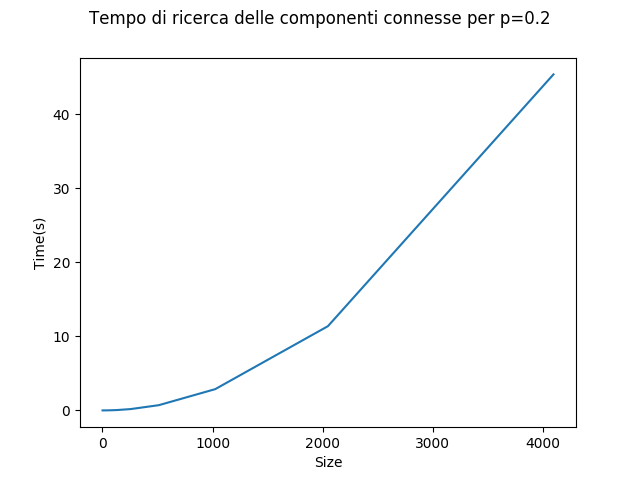
\includegraphics[width=\textwidth]{cc_time_p=02}
        \label{fig:ccs_time_p=02}
    \end{subfigure}
    \quad
    \begin{subfigure}[b]{0.45\linewidth}
        \centering
        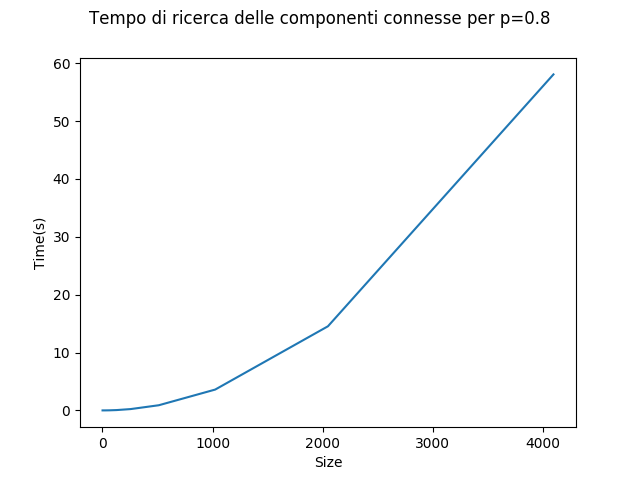
\includegraphics[width=\textwidth]{cc_time_p=08}
        \label{fig:ccs_time_p=08}
    \end{subfigure}
\end{figure}
\newpage
\subsection{MST}
\textbf{Tempi di esecuzione}
\begin{table}[H]
\centering
\caption{Tempo di esecuzione(s)}
\label{tab:mst_time}
\begin{tabular}{|l|l|l|l|l|l|} 
\cline{2-6}
\multicolumn{1}{l|}{} & p = 0.2 & p = 0.4 & p = 0.6 & p= 0.8 & p = 1   \\ 
\hline
16                    & 0.0016  & -       & 0.0020  & 0.0021 & 0.0024  \\
32                    & 0.0061  & 0.0070  & 0.0099  & 0.0085 & 0.0092  \\
64                    & 0.048   & 0.028   & 0.031   & 0.034  & 0.039   \\
128                   & 0.096   & 0.11    & 0.14    & 0.14   & 0.17    \\
256                   & 0.37    & 0.43    & 0.49    & 0.54   & 0.62    \\
512                   & 1.53    & 1.76    & 2.03    & 2.26   & 2.47    \\
1024                  & 6.17    & 7.14    & 8.09    & 9.03   & 10.1    \\
2048                  & 24.8    & 28.7    & 32.7    & 36.6   & 40.4    \\
4096                  & 99.5    & 115.4   & 132.5   & 148.1  & 164.4   \\
\hline
\end{tabular}
\end{table}

\begin{figure}[H]
    \centering
    \begin{subfigure}[b]{0.45\linewidth} 
        \centering
        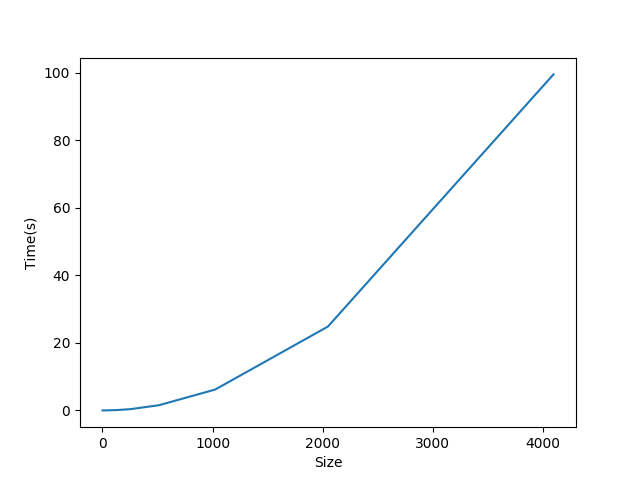
\includegraphics[width=\textwidth]{krusk_time_p=02}
        \label{fig:krusk_time_p=02}
    \end{subfigure}
    \quad
    \begin{subfigure}[b]{0.45\linewidth}
        \centering
        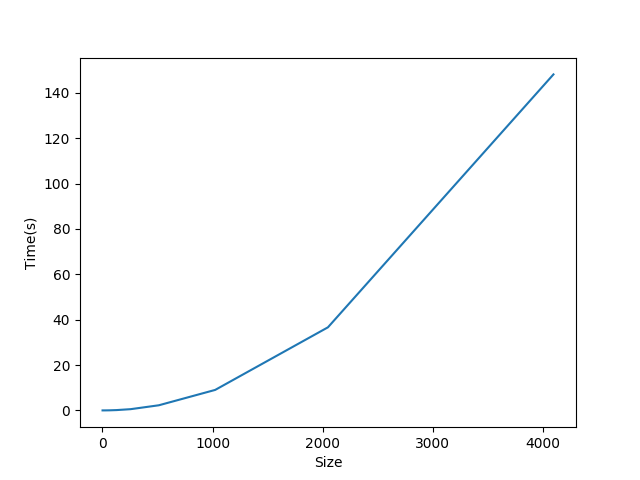
\includegraphics[width=\textwidth]{krusk_time_p=08}
        \label{fig:krusk_time_p=08}
    \end{subfigure}
\end{figure}

\textbf{Peso MST}\\

\begin{table}[H]
\centering
\caption{Peso}
\label{tab:mst_weight}
\begin{tabular}{|l|l|l|l|l|l|} 
\cline{2-6}
\multicolumn{1}{l|}{} & p = 0.2 & p = 0.4 & p = 0.6 & p= 0.8 & p = 1  \\ 
\hline
16                    & 55      & -       & 30      & 19     & 25     \\
32                    & 64      & 42      & 41      & 31     & 32     \\
64                    & 107     & 65      & 63      & 63     & 63     \\
128                   & 134     & 129     & 127     & 127    & 127    \\
256                   & 256     & 255     & 255     & 255    & 255    \\
512                   & 511     & 511     & 511     & 511    & 511    \\
1024                  & 1023    & 1023    & 1023    & 1023   & 1023   \\
2048                  & 2047    & 2047    & 2047    & 2047   & 2047   \\
4096                  & 4095    & 4095    & 4095    & 4095   & 4095   \\
\hline
\end{tabular}
\end{table}

\begin{figure}[H]
    \centering
    \begin{subfigure}[b]{0.45\linewidth} 
        \centering
        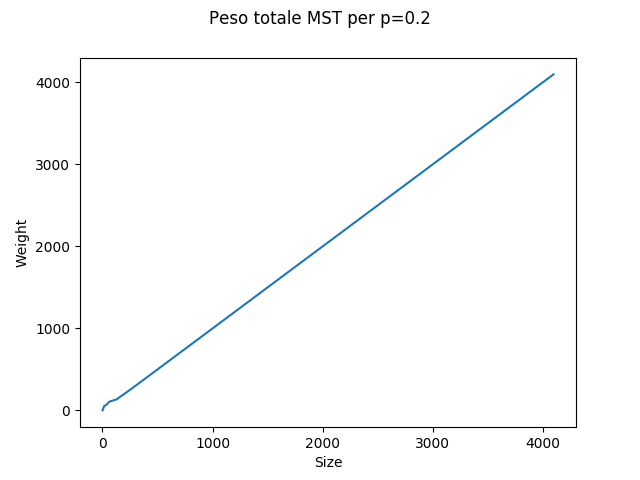
\includegraphics[width=\textwidth]{krusk_Weight_p=02}
        \label{fig:krusk_Weight_p=02}
    \end{subfigure}
    \quad
    \begin{subfigure}[b]{0.45\linewidth}
        \centering
        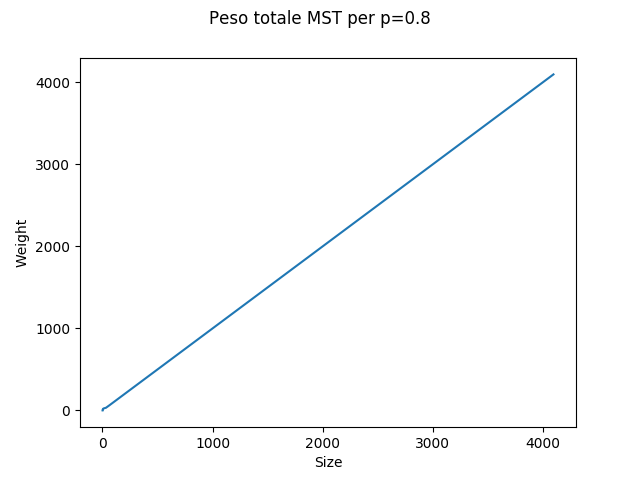
\includegraphics[width=\textwidth]{krusk_Weight_p=08}
        \label{fig:krusk_Weight_p=08}
    \end{subfigure}
\end{figure}

\textbf{Altezza MST}\\
\begin{table}[H]
\centering
\caption{Altezza}
\label{tab:mst_height}
\begin{tabular}{|l|l|l|l|l|l|} 
\cline{2-6}
\multicolumn{1}{l|}{} & p = 0.2 & p = 0.4 & p = 0.6 & p= 0.8 & p = 1  \\ 
\hline
16                    & 5       & -       & 5       & 4      & 3      \\
32                    & 8       & 7       & 7       & 6      & 5      \\
64                    & 6       & 10      & 6       & 8      & 6      \\
128                   & 12      & 9       & 6       & 8      & 8      \\
256                   & 13      & 9       & 9       & 8      & 6      \\
512                   & 13      & 10      & 10      & 8      & 8      \\
1024                  & 14      & 10      & 10      & 8      & 8      \\
\hline
\end{tabular}
\end{table}

\begin{figure}[H]
    \centering
    \begin{subfigure}[b]{0.45\linewidth} 
        \centering
        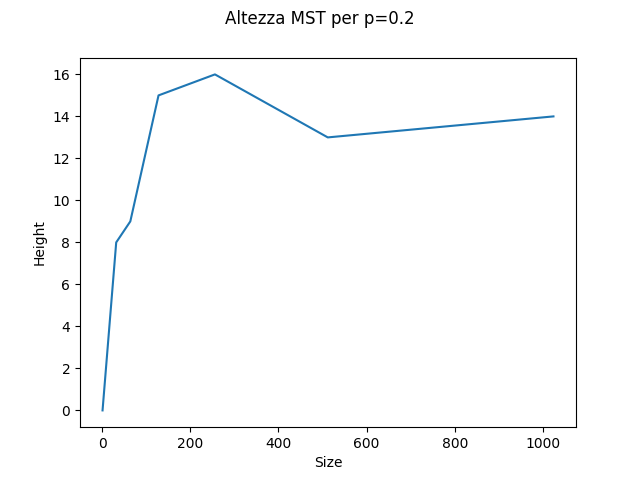
\includegraphics[width=\textwidth]{krusk_height_p=02}
        \label{fig:quick_casuale}
    \end{subfigure}
    \quad
    \begin{subfigure}[b]{0.45\linewidth}
        \centering
        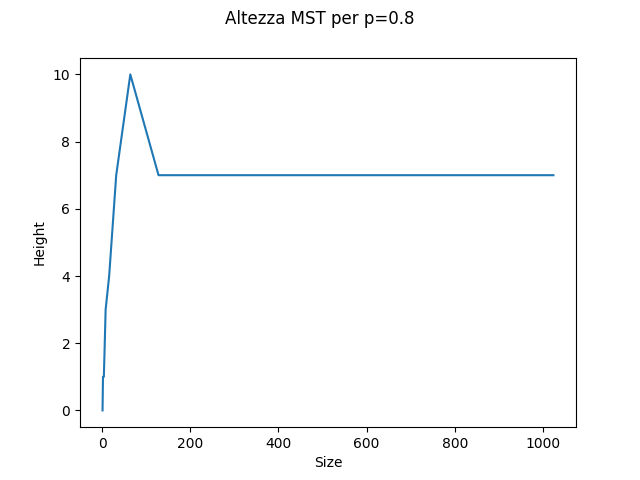
\includegraphics[width=\textwidth]{krusk_height_p=08}
        \label{fig:quick_best}
    \end{subfigure}
\end{figure}
\newpage
\section{Analisi e conclusioni}
Dagli esperimenti emerge che molto spesso nel grafo generato si ha una sola componente connessa.\\
Questo è particolarmente vero quando il numero di vertici del grafo è superiore a 10-20, infatti anche se la probabilità di avere un collegamento tra due nodi è abbastanza bassa in qualche modo sarà generato un cammino che collega qualsiasi coppia di nodi, più o meno lungo.\\
I tempi di esecuzione di questo algoritmo sono quelli attesi ovvero più che lineare rispetto al numero di archi, cioè alla dimensione e alla probabilità di collegamento dei nodi.\\
\\
Un comportamento molto simile lo ha anche il tempo di ricerca dell'MST, anche se le sue costanti sono più alte.\\
Il peso totale dell'MST è lineare rispetto al numero di nodi,questo ha però un comportamento particolare al variare della probabilità di presenza di archi.\\
Infatti da qualche centinaio di nodi in su e a parità del loro numero, nonostante due grafi siano più o meno popolati di archi(p diversi) il peso dei due MST è molto vicino, se non identico.\\
Infine è possibile osservare come l'altezza dell'MST inizialmente aumenta con l'aumentare del numero di nodi, questo comportamento però si attenua su grafi di dimensioni maggiori dove l'altezza si inizia a stabilizzare attorno a 10 o 8, a seconda di p.\\
Ciò significa che anche aumentando notevolmente il numero di nodi la lunghezza dei cammini  tra qualsiasi coppia di nodi nell'MST resta ragionevole.\\
 
\end{document}